\documentclass[a4paper, 11pt]{article}
\usepackage{epsf}
\usepackage{epsfig}
\usepackage{amsmath}
\usepackage{amssymb}
\usepackage{theorem}
\usepackage{alltt}
\usepackage{times}
\usepackage{helvet}
\usepackage{xspace}
\topmargin=15pt
\oddsidemargin=20pt
\headsep=20pt
\footskip=30pt
\textheight=600pt
\textwidth=400pt

\newcommand{\bm}{{\tt Batman}\xspace}
\renewcommand{\familydefault}{\sfdefault}

\begin{document}
\title{{\tt Batman}: a tool for quantifying DNA methylation.}
\author{Manual by Thomas A. Down \\ 
  {\it thomas.a.down@googlemail.com}}
\date{Version 0.2.3 [20080422]}
\maketitle

\begin{abstract}
{\tt Batman} is a statistical tool for analyzing MeDIP experiments and giving a
quantitative read-out of methylation state in a region.  It can be applied to
large datasets, including genome-wide datasets produced using large tiling arrays
or new high-throughput sequencing methods.
\end{abstract}

\section{Theory}

\bm is a new tool used in this study to transform the output signal
from Methyl-DNA immunoprecipitation experiments into quantitative
measures of DNA methylation.  The core principle of the Batman
algorithm is to model the effects of varying density of CpG
dinucleotides, and the effect this has on MeDIP enrichment of DNA
fragments.  Here, we'll consider MeDIP experiments assayed using
tiling microarrays (MeDIP/chip), but similar principles could be
applied to alternative assays, for example those using new
high-throughput sequencing technologies.

To model the MeDIP/chip signal, we first define a coupling factor, $C_{cp}$
between a microarray probe, $p$ and any nearby CpG dinucleotide $c$.
This is an estimate of the fraction of DNA fragments hybridizing to the probe
which will contain the given CpG, which clearly depends on the length
distribution of the DNA fragments.  In this study, fragments of between
400 and 700bp in length were selected.  We assume that the fragment
length distribution is fairly uniform within this range, and estimate
the distribution of $C_{cp}$ depending on the distance between $c$ and
$p$ accordingly.
For any given probe, we can define a total CpG influence parameter,
$C_{tot}$ as the sum of coupling factors between that probe and all
CpGs.  Now, the signal from the
MeDIP channel of the microarray experiment depends on the degree of
enrichment of DNA fragments overlapping that probe, which in turn
depends on the amount of antibody binding, and thus to the number of
methylated CpGs on those fragments.  For fully methylated DNA, we
might expect some transformation of the array output of each probe, $A_p$, to scale
linearly with $C_{tot}$.  For fully unmethylated DNA, $A_p$ and $C_{tot}$
should, of course, be independent.  

Now, considering some real MeDIP/chip data, plotting $C_{tot}$ against a
common statistic for 2-channel microarrays ($\log_2$ ratio of the
channels) gives a complex plot as shown in figure \ref{example.calibrate}.  Following prior
observations [ref] that most regions of low CpG density are
constitutively methylated while most regions of high CpG density (CpG
islands) are constitutively unmethylated, we focus on the low-$C_{tot}$
section of this plot.  In this region, the trend (calculated by
discarding the highest and lowest 20\% of the data in a unit $C_{tot}$ interval and
taking the mean of the central portion) of the log-ratio
statistic increases linearly in proportion to $C_{tot}$.  We therefore
propose that this statistic is a good approximation to our hypothetical
$A$.  For each array in our study, we fitted a linear model of $A$ against
$C_{tot}$, only considering probes with $C_{tot }\leq 10$, and recorded the
slope ($r$) and $A_p$-intercept ($A_{base}$) of this model. 
We also need to estimate
the inverse variance, $\nu$, of $A$ around its mean.  In one study on Nimblegen arrays, we found thta
this was approximately 0.1, and was fairly consistent across many arrays.

For each CpG dinucleotide in the genome, $c$, let $m_c$ represent the fraction
of chromosomes in the sample on which it is methylated.  Since many samples used in
MeDIP studies are hetrogenous -- containing multiple cell-types -- we consider $m_c$ as
a continuous variable.  Given our model, the complete dataset from a
MeDIP/chip experiment, $A$, varies as:

\begin{equation}
f(A | m) = \prod_p {\mathcal G}(A_p | A_{base} + r \sum_{c}{C_{cp}m_c}, \nu^{-1})
\end{equation}

where ${\mathcal G(x | \mu, \sigma^2})$ is a Gaussian p.d.f.
We can now use any standard Bayesian inference approach to find $f(m |A)$,
the posterior distribution of the methylation state parameters
given the array data, and thus generate quantitative methylation
profile information.

In order to reduce the computational cost of analyzing regions with very high
CpG density, we take advantage of the fact that CpG methylation state is
generally very highly correlated over a scale of hundreds of bases [HEP
reference].  Instead of modeling every CpG individually, we grouped together
all CpGs in 50bp windows and assumed that they would have the same methylation
state.

Our implementation of the Batman model uses Nested Sampling (http://www.inference.phy.cam.ac.uk/bayesys/), a recently-described
and highly robust Monte Carlo technique, to solve this inference problem.  For each
tiled region of the genome, we use a Nested Sampler to generate 100 independent
samples from $P(m | A)$.  We then summarize the most likely methylation state in 100bp
windows.

\section{Installation}

{\tt Batman} is a Java program and should run on any computer with a reasonable
Java implementation (requires Java 5 or later).  If your computer does not include
pre-installed Java, see:

\begin{alltt}    http://java.sun.com/\end{alltt}

The instructions here assume that you are using a Unix-like system (Linux, Mac OS X,
{\it etc.}, but we do have reports that {\tt Batman} can be used under Microsoft
Windows.  In addition to the {\tt Batman} software, you will need Apache ANT:

\begin{alltt}    http://ant.apache.org/\end{alltt}

and the MySQL database server:

\begin{alltt}    http://www.mysql.com/\end{alltt}

You can either install MySQL locally on the same machine where you install {\tt Batman},
or connect to a separate database server on your local network.  If you have a large
amount of data to analyze, several computers running {\tt Batman} can successfully
share a single MySQL server.  In principle, it should be possible to run {\tt Batman}
with other database servers, but this has not been tested.

Finally, you'll need the MySQL database connector:

\begin{alltt}    http://www.mysql.com/products/connector/j/\end{alltt}

To install the {\tt Batman} software, unpack the source code (probably called something
like {\tt batman.tar.gz}), change into the {\tt batman} directory, then type:

\begin{alltt}     ant\end{alltt}

The compiled code will go in {\tt lib/batman.jar}.  You'll then need to set your
{\tt CLASSPATH} environment variable to point to all the {\tt .jar} files in the
{\tt lib} directory, and also to the MySQL Connector/J {\tt .jar} file.

All the \bm tools are run with a command line like:

\begin{alltt}   java <java options> batman.SomeToolApplication <batman options>\end{alltt}

There are several Java options which may be helpful:

\begin{itemize}
\item{{\tt -server} will speed up execution of long-running jobs.}
\item{{\tt -XmxNNNNM} will set a memory limit of NNNN megabytes.}
\end{itemize}

On some platforms, Java's default memory limit is ridiculously low and you'll see
{\tt OutOfMemoryError} messages when you try to run \bm.  If so, try a larger
memory limit.  {\tt -Xmx1500M} works well.

\section{Analyzing a dataset}

This protocol assumes that your dataset is broken up into small blocks (regions of
interest, subsequently ROIs), each represented by a small number (typically <100)
probes on a microarray.  If this is not true for your dataset, consult the section
on tilepaths, below.

The default database-loading tools assume that you have your data formatted in
GFF2 format:

\begin{alltt}    http://www.sanger.ac.uk/Software/formats/GFF/\end{alltt}

Most other formats can be converted into GFF using fairly straightforward
scripts.

\subsection{Identify your database server}

To run {\tt Batman}, you'll need to connect to a MySQL database server using
both the {\tt mysql} administration tool, and many of the {\tt Batman} programs.
If you haven't used MySQL before, see:

\begin{alltt}    http://www.mysql.com/\end{alltt}

for instructions on installation and administration.  You'll need to know:

\begin{itemize}
\item{Your database server username}
\item{Your database server password}
\item{The name of the computer where MySQL is installed (if it isn't your local machine)}
\end{itemize}

The {\tt Batman} tools all take some standard options to specify how to connect
to the database:

\begin{alltt}java batman.Tool -dbURL jdbc:mysql://database-server/batman_test 
                    -dbUser <username> -dbPass <password>\end{alltt}

you can give the hostname of a server where MySQL is installed, or {\tt localhost}
if it's on the same machine that you're using to run \bm.

\subsection{Initialize the \bm database}

First, you'll need to create a database on your database server.  You can do this using
the command line MySQL monitor:

\begin{alltt}    mysql -u<user> -p<passwd>
    create database batman_test\end{alltt}

You can call your database whatever you like, but for the purposes of this tutorial
we'll assume it's called {\tt batman\_test}.  You must now initialize it:

\begin{alltt}    mysql -u<user> -p<passwd> batman_test <schema.sql
    mysql -u<user> -p<passwd> batman_test <flat-400-700.sql\end{alltt}

(The second step isn't needed if you're supplying your own DNA fragment length
distribution).

\subsection{Register the experiments you'll be analyzing}

For each experimental dataset ({\it e.g.} microarray), that you intend to analyze,
you should register it with {\tt Batman} using a command like:

\begin{alltt}java batman.AddExptApplication <DB options>
                    -expt SP1A
                    -array 12345
                    -tissue Sperm
                    -sample SP1
                    -cy3 IP -cy5 INPUT\end{alltt}

The {\tt -expt} tag is a string that will be used throughout the {\tt Batman}
system to identify that array.  You can (optionally) specify the meanings of
each channel of a two-channel array (IP, INPUT, or Unknown) using the {\tt -cy3}
and {\tt -cy5} options.

\subsection{Register the array design}

The array design ({\it i.e.} complete list of probes, with their genomic locations)
should be provided as a GFF file.  Each line in the file represents one probe,
and has two group attributes, specifying the probe ID and the ROI ID.  For example:

\begin{alltt}22  probe   array   50  75  .   .   .   probe PROBE1; ROI ROI1\end{alltt}

defines a probe called ``PROBE1'' associated with ROI ``ROI1''.  Every probe must be
associated with exactly one ROI.  \bm is quite flexible about the exact definition of
an ROI -- basically, it can be any cluster of probes.  In the extreme case of a whole-genome
tiling array, you should call all the probes on one chromosome an ROI.

To load the array design:

\begin{alltt}    java batman.LoadProbesApplication <DB options> probes.gff\end{alltt}

Currently, we only recommend loading one array design into a \bm database.  If you
are working on multiple projects with different array designs, please create a new
database for each project.

\subsection{Load the array data}

Array data is also currently specified in GFF format.  The actual data (generally
a log-ratio) should be included in the score field.  Note that the {\tt probe}
attribute is required.

\begin{alltt}22  ratio   array   50  75  -2.5   .   .   probe PROBE1\end{alltt}

If you have multiple arrays, you should load each one separately.

It would be fairly straightforward to add loaders for other data formats.  Please
contact the author if you have any specific requests, or take a look at the source
file {\tt batman/LoadProbes.java} to get any idea of what is involved in rolling
your own.

\subsection{Load the genome sequence}

\bm needs access to a reference genome sequence in order to determine the distribution
of CpG dinucleotides.  Currently, genome sequence is read from the \bm database.  To
load a genome sequence, ensure that it is formatted in FASTA format, then:

\begin{alltt}    java batman.LoadGenomeTilesApplication <database options>
         -seqFile genome.fa\end{alltt} 

You can issue this command multiple times if your genome data is split into
several files ({\it e.g.} one per chromosome).

Future versions of \bm may allow sequence data to be fetched from Ensembl databases
instead.  Please contact the author if this would be useful to you.

\subsection{Calibrate the \bm model}

Before any data can be analyzed, it is necessary to calibrate each array by
estimating how much extra array signal is produced by each methylated CpG.  In
the simplest case, you can do this by typing:

\begin{alltt}java batman.CalibrateApplication <DB options>
        -expt <experiment ID>
        -writeDB\end{alltt}

This will compare array signal with CpG density, fit a linear model, and write
the results back to the database.  In principle, this is all that is needed
to calibrate \bm.  However, the calibration step is a good point to check that
each of your arrays is giving sensible results.  To do this, add the following
options to the {\tt CalibrateApplication} command line:

\begin{alltt}-writeScatter scatter.dat -writeTrend trend.dat\end{alltt}

Plotting the resulting data should give a plot similar to figure \ref{example.calibrate}.  If you
use {\tt gnuplot} try:

\begin{alltt}set xlabel 'log2 ratio'
set ylabel 'Total CpG influence'
plot 'scatter.dat' ti 'MeDIP data', 
     'trend.dat' ti 'Means of central portion' with linespoints lw 2\end{alltt}

If the resulting plot looks substantially different from figure \ref{example.calibrate}, it may mean
that there is a problem with your data, or that it has not been processed
correctly.  If you're asking for advice about a particular array, it would be
extremely helpful if you include a ``calibration plot'' produced in this way.

If you {\it just} want to do array quality control without writing anything
to the database, you can omit the {\tt -writeDB} option.

\begin{figure}[!bth]
\begin{center}
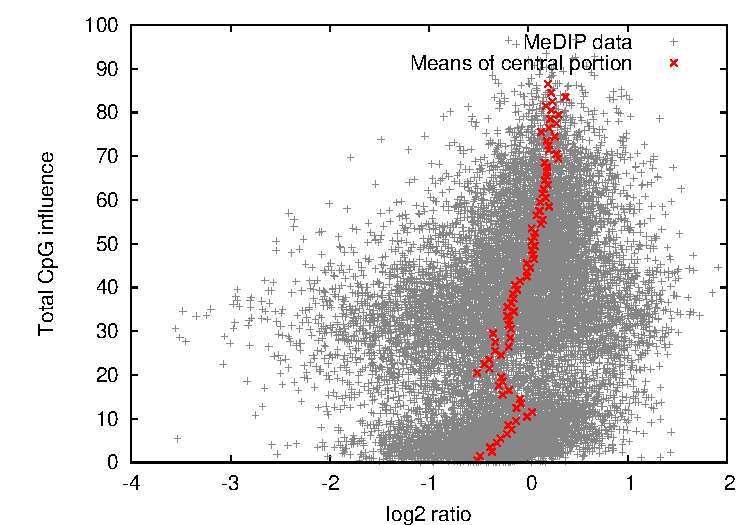
\includegraphics[scale=0.66]{calibrate.pdf}
\caption{Example \bm calibration plot.}
\label{example.calibrate}
\end{center}
\end{figure}

\subsection{Sample methylation states from the \bm model}

First of all, generate one or more text files containing lists of ROI identifiers.
This could be a full list of all the ROIs on your array, but doesn't have to be.
In particular, if you want to use multiple CPUs to run \bm, you can split your ROI
list into equal-sized chunks and run multiple instances of \bm.  One database
server can typically support several \bm instances.

To run the \bm model:

\begin{alltt}java -server batman.SampleMethStatesApplication <DB options> 
           <array options> 
           -roiSamples roi-list-file.txt 
           | gzip -c >batman-samples.xml.gz\end{alltt}

You'll often have multiple arrays from the same experiment, and these should
normally be analyzed together to improve the confidence of the final calls.
You can select any subset of arrays in the database by providing
one or more {\tt -expt} options on the command line {\it e.g.}:

\begin{alltt}-expt SP1A -expt SP1B -expt SP2A\end{alltt}

Alternatively, if you put something meaningful into the {\tt -tissue}
field when registering your arrays, you can just do:

\begin{alltt}-tissue Sperm\end{alltt}

You'll notice that in the example, the output from {\tt SampleMethStatesApplication} is piped through {\tt gzip}.  For any
serious-sized dataset, {\tt SampleMethStatesApplication} produces a
huge amount of output, so -- except perhaps for test purposes --
you'll always want to keep it in compressed format.  The output is
reduced into a much more compact for by the summarization step.  Once
you're happy with your summarized results, you'll probably want to
delete the sample files.

\subsection{Summarize methylation states to generate the final calls}

The ``sample'' files generated by \bm contain a large set of plausible
methylation states for each region.  Exactly how similar these states
are to one another depends on the quantity and quality of data available
in that region.  For most purposes, you'll actually want a single estimate
of the likely methylation state at that position, and perhaps an estimate
of how confident you can be that this is actually the correct value.

To use the default \bm summarization, strategy:

\begin{alltt}java batman.SummarizeApplication 
    batman-samples.xml.gz
    >batman-results.gff\end{alltt}

The output is in GFF format.  For each window, a score is given which represents 
a likely fraction of methylation (actually the median of all sampled methylation
states in that window) and the inter-quartile range is given as an estimate of
confidence.  Several other summarization strategies have been used in the past.

By necessity, \bm infers methylation levels for sequences some distance from
the tiled regions on your arrays.  However, the quality of these calls obviously
drops off rapidly as you move away from the tiled regions.  For this reason, it
is often better to trim the results back to ROI boundaries.  This can be accomplished
by using the {\tt -trim} option.  ROI boundaries are read from the \bm database,
and you must specify database connection options as normal when using the {\tt -trim}
option.

\section{Custom coupling profiles}

TODO

\section{Tilepaths}

\bm can also be used to analyse large regions of the genome that are covered by probes
from a tiling array.  To analyse such datasets, you should load your data as normal, defining
each tiled region as one ROI.  Potentially, a tilepath ROI could cover an entire chromosome.
If your dataset includes tiled regions on different sequences, these must be given different
names.

Having loaded the data and calibrated as normal, you can analyse an ROI named {\tt TILEDREGION}
with a command like:

\begin{alltt}java -server batman.SampleMethStatesApplication <DB options> 
           <array options> 
           -tilepathSamples TILEDREGION
           | gzip -c >batman-samples.xml.gz\end{alltt}

\bm will split your tiled regions into chunks.  The exact behaviour can be tuned using
the {\tt -tilepathTile}, {\tt -tilepathStep}, and {\tt -tilepathFlank} options.  The output
can be converted to GFF using the Summarize tool as normal.

\section{MeDIP-Seq}

{\tt Batman} can also be used for whole-genome methylation profiling using a
MeDIP + DNA sequencing protocol.  Contact the author for more information.

\section{Acknowledgements}

Thanks to Vardhman Rakyan, Stephan Beck, Natalie Thorne, and James Prendergast for
helpful advise and comments during the development of this software.

\end{document}

